\documentclass{article}
\usepackage{graphicx} % new way of doing eps files
\usepackage{listings} % nice code layout
\usepackage[usenames]{color} % color
\usepackage{float}
\definecolor{listinggray}{gray}{0.9}
\definecolor{graphgray}{gray}{0.7}
\definecolor{ans}{rgb}{1,0,0}
\definecolor{blue}{rgb}{0,0,1}
% \Verilog{title}{label}{file}
\newcommand{\Verilog}[3]{
	\lstset{language=Verilog}
	\lstset{backgroundcolor=\color{listinggray},rulecolor=\color{blue}}
	\lstset{linewidth=\textwidth}
	\lstset{commentstyle=\textit, stringstyle=\upshape,showspaces=false}
	\lstset{frame=tb}
	\lstinputlisting[caption={#1},label={#2}]{#3}
}


\author{Steve Potter}
\title{Lab 2 - Program Counter}

\begin{document}
	\maketitle
	
	\section{Executive Summary}
	The goal of this lab is to create an adder module and a mux module.  These modules will initially be used in the Fetch stage of our 64-bit ARMv8 processor.  The adder will be used to increment the Program Counter (PC).  The incremented PC will be used for sequential program execution.  The mux will be used to set the PC to either the incremented PC or to a branch address.  This selection will be based on the mux control line, which specifies whether the program should branch or continue running sequentially.  The module works correctly as shown by the test report below
	
	\section{Test Report}
	To verify operation of these two modules, this lab requires two separate test benches.
	\begin{enumerate}
		\item Adder Test Bench
		\item Mux Test Bench
	\end{enumerate}
	
	\begin{figure}[H]
		\begin{center}
			\caption{Expected Results of the adder test.}\label{fig:ert_addertest}
			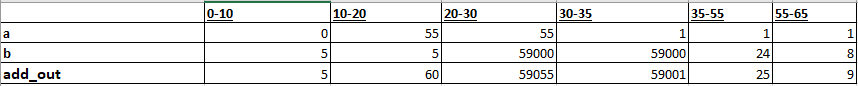
\includegraphics[width=1.0\textwidth]{../images/ert_adder_test.png}
		\end{center}
	\end{figure}
	
	\begin{figure}[H]
		\begin{center}
			\caption{Timing diagram for the adder test.}\label{fig:addertest}
			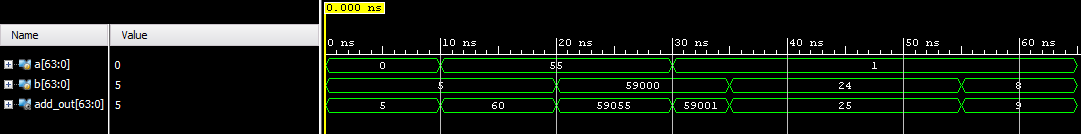
\includegraphics[width=1.0\textwidth]{../images/adder_test.png}
		\end{center}
	\end{figure}
	
	\begin{figure}[H]
		\begin{center}
			\caption{Expected Results of the mux test.}\label{fig:ert_muxtest}
			\includegraphics[width=1.0\textwidth]{../images/ert_mux_test.png}
		\end{center}
	\end{figure}
	
	\begin{figure}[H]
		\begin{center}
			\caption{Timing diagram for the mux test.}\label{fig:muxtest}
			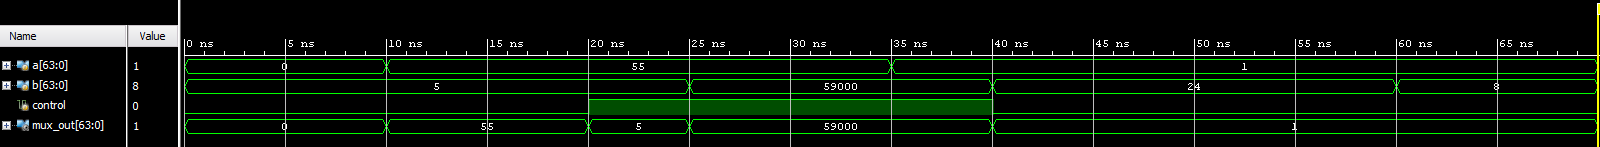
\includegraphics[width=1.0\textwidth]{../images/mux_test.png}
		\end{center}
	\end{figure}
	
	
	\section{Code Appendix}
	\Verilog{Verilog code for testing the adder.}{code:addertest}{../code/0_common/adder_test.v}
	
	\Verilog{Verilog code for testing the mux.}{code:muxtest}{../code/0_common/mux_test.v}
		
	\Verilog{Verilog code for the adder.}{code:addertest}{../code/0_common/adder.v}
	
	\Verilog{Verilog code for the mux.}{code:addertest}{../code/0_common/mux.v}

	
\end{document} 